% File: figures/power_configurations_barchart.tex
% Grafico a barre per confronto configurazioni sistemi di alimentazione
% Per uso con \input{} nel documento principale

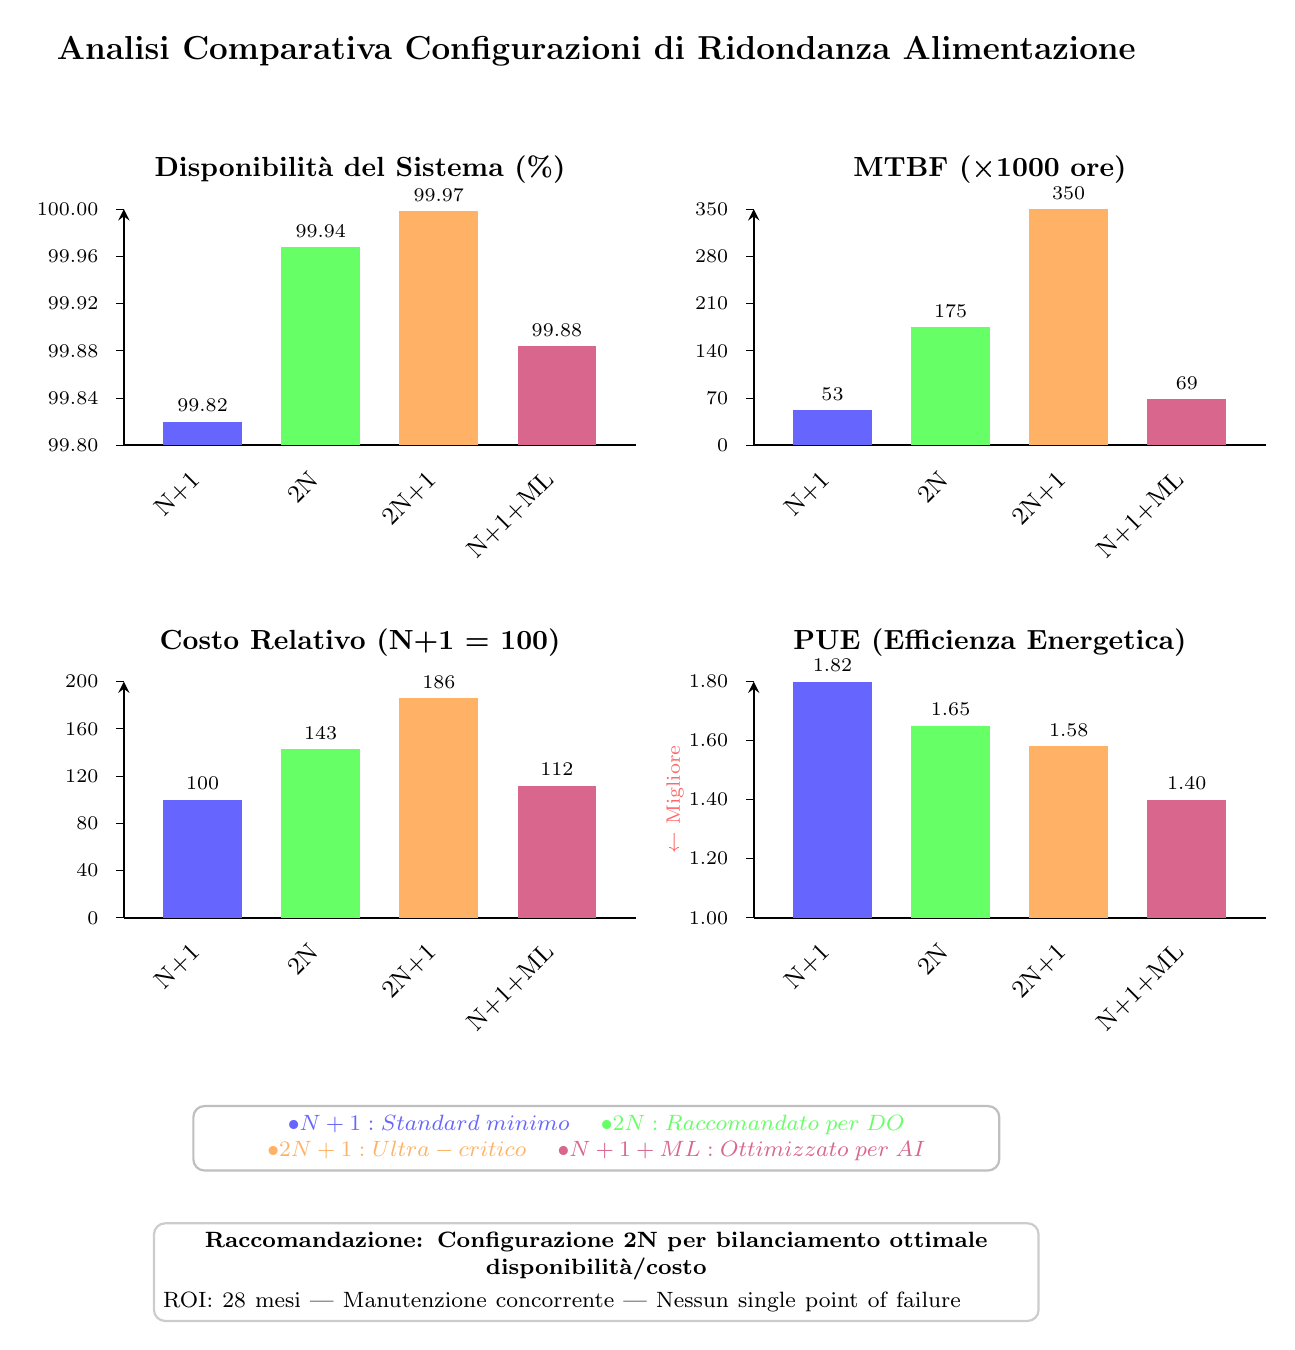
\begin{tikzpicture}
[
    % Stili per le barre
    barN1/.style={fill=blue!60},
    bar2N/.style={fill=green!60},
    bar2N1/.style={fill=orange!60},
    barML/.style={fill=purple!60},
    % Stile per gli assi
    axis/.style={thick, ->, >=stealth},
    % Stile per le etichette
    label/.style={font=\small},
    value/.style={font=\scriptsize},
    title/.style={font=\large\bfseries}
]

% === TITOLO ===
\node[title] at (6,11) {Analisi Comparativa Configurazioni di Ridondanza Alimentazione};

% === GRAFICO 1: DISPONIBILITÀ ===
\begin{scope}[shift={(0,6)}]
    % Titolo del grafico
    \node[font=\normalsize\bfseries] at (3,3.5) {Disponibilità del Sistema (\%)};
    
    % Asse Y
    \draw[axis] (0,0) -- (0,3);
    \foreach \y/\val in {0/99.80, 0.6/99.84, 1.2/99.88, 1.8/99.92, 2.4/99.96, 3/100.00} {
        \draw (0,\y) -- (-0.1,\y);
        \node[value, left] at (-0.2,\y) {\val};
    }
    
    % Asse X
    \draw[thick] (0,0) -- (6.5,0);
    
    % Barre
    % N+1: 99.82%
    \fill[barN1] (0.5,0) rectangle (1.5,0.3) node[value, above] at (1,0.3) {99.82};
    
    % 2N: 99.94%
    \fill[bar2N] (2,0) rectangle (3,2.52) node[value, above] at (2.5,2.52) {99.94};
    
    % 2N+1: 99.97%
    \fill[bar2N1] (3.5,0) rectangle (4.5,2.97) node[value, above] at (4,2.97) {99.97};
    
    % N+1+ML: 99.88%
    \fill[barML] (5,0) rectangle (6,1.26) node[value, above] at (5.5,1.26) {99.88};
    
    % Etichette X
    \node[label, rotate=45, anchor=east] at (1,-0.3) {N+1};
    \node[label, rotate=45, anchor=east] at (2.5,-0.3) {2N};
    \node[label, rotate=45, anchor=east] at (4,-0.3) {2N+1};
    \node[label, rotate=45, anchor=east] at (5.5,-0.3) {N+1+ML};
\end{scope}

% === GRAFICO 2: MTBF ===
\begin{scope}[shift={(8,6)}]
    % Titolo del grafico
    \node[font=\normalsize\bfseries] at (3,3.5) {MTBF (×1000 ore)};
    
    % Asse Y
    \draw[axis] (0,0) -- (0,3);
    \foreach \y/\val in {0/0, 0.6/70, 1.2/140, 1.8/210, 2.4/280, 3/350} {
        \draw (0,\y) -- (-0.1,\y);
        \node[value, left] at (-0.2,\y) {\val};
    }
    
    % Asse X
    \draw[thick] (0,0) -- (6.5,0);
    
    % Barre
    % N+1: 52.560
    \fill[barN1] (0.5,0) rectangle (1.5,0.45) node[value, above] at (1,0.45) {53};
    
    % 2N: 175.200
    \fill[bar2N] (2,0) rectangle (3,1.5) node[value, above] at (2.5,1.5) {175};
    
    % 2N+1: 350.400
    \fill[bar2N1] (3.5,0) rectangle (4.5,3) node[value, above] at (4,3) {350};
    
    % N+1+ML: 69.141
    \fill[barML] (5,0) rectangle (6,0.59) node[value, above] at (5.5,0.59) {69};
    
    % Etichette X
    \node[label, rotate=45, anchor=east] at (1,-0.3) {N+1};
    \node[label, rotate=45, anchor=east] at (2.5,-0.3) {2N};
    \node[label, rotate=45, anchor=east] at (4,-0.3) {2N+1};
    \node[label, rotate=45, anchor=east] at (5.5,-0.3) {N+1+ML};
\end{scope}

% === GRAFICO 3: COSTO RELATIVO ===
\begin{scope}[shift={(0,0)}]
    % Titolo del grafico
    \node[font=\normalsize\bfseries] at (3,3.5) {Costo Relativo (N+1 = 100)};
    
    % Asse Y
    \draw[axis] (0,0) -- (0,3);
    \foreach \y/\val in {0/0, 0.6/40, 1.2/80, 1.8/120, 2.4/160, 3/200} {
        \draw (0,\y) -- (-0.1,\y);
        \node[value, left] at (-0.2,\y) {\val};
    }
    
    % Asse X
    \draw[thick] (0,0) -- (6.5,0);
    
    % Barre
    % N+1: 100
    \fill[barN1] (0.5,0) rectangle (1.5,1.5) node[value, above] at (1,1.5) {100};
    
    % 2N: 143
    \fill[bar2N] (2,0) rectangle (3,2.145) node[value, above] at (2.5,2.145) {143};
    
    % 2N+1: 186
    \fill[bar2N1] (3.5,0) rectangle (4.5,2.79) node[value, above] at (4,2.79) {186};
    
    % N+1+ML: 112
    \fill[barML] (5,0) rectangle (6,1.68) node[value, above] at (5.5,1.68) {112};
    
    % Etichette X
    \node[label, rotate=45, anchor=east] at (1,-0.3) {N+1};
    \node[label, rotate=45, anchor=east] at (2.5,-0.3) {2N};
    \node[label, rotate=45, anchor=east] at (4,-0.3) {2N+1};
    \node[label, rotate=45, anchor=east] at (5.5,-0.3) {N+1+ML};
\end{scope}

% === GRAFICO 4: PUE (EFFICIENZA) ===
\begin{scope}[shift={(8,0)}]
    % Titolo del grafico
    \node[font=\normalsize\bfseries] at (3,3.5) {PUE (Efficienza Energetica)};
    
    % Asse Y
    \draw[axis] (0,0) -- (0,3);
    \foreach \y/\val in {0/1.00, 0.75/1.20, 1.5/1.40, 2.25/1.60, 3/1.80} {
        \draw (0,\y) -- (-0.1,\y);
        \node[value, left] at (-0.2,\y) {\val};
    }
    
    % Nota: valori più bassi sono migliori
    \node[value, text=red!60, rotate=90] at (-1,1.5) {← Migliore};
    
    % Asse X
    \draw[thick] (0,0) -- (6.5,0);
    
    % Barre (invertite - più basso è meglio)
    % N+1: 1.82
    \fill[barN1] (0.5,0) rectangle (1.5,3) node[value, above] at (1,3) {1.82};
    
    % 2N: 1.65
    \fill[bar2N] (2,0) rectangle (3,2.44) node[value, above] at (2.5,2.44) {1.65};
    
    % 2N+1: 1.58
    \fill[bar2N1] (3.5,0) rectangle (4.5,2.18) node[value, above] at (4,2.18) {1.58};
    
    % N+1+ML: 1.40
    \fill[barML] (5,0) rectangle (6,1.5) node[value, above] at (5.5,1.5) {1.40};
    
    % Etichette X
    \node[label, rotate=45, anchor=east] at (1,-0.3) {N+1};
    \node[label, rotate=45, anchor=east] at (2.5,-0.3) {2N};
    \node[label, rotate=45, anchor=east] at (4,-0.3) {2N+1};
    \node[label, rotate=45, anchor=east] at (5.5,-0.3) {N+1+ML};
\end{scope}

% === LEGENDA ===
\node[draw=gray!50, thick, rounded corners] at (6,-2.8) {
    \begin{minipage}{10cm}
    \centering\footnotesize
    \textcolor{blue!60}{$\bullet  N+1: Standard \; minimo$} \quad
    \textcolor{green!60}{$\bullet  2N: Raccomandato \; per \; DO$} \quad
    \textcolor{orange!60}{$\bullet  2N+1: Ultra-critico$} \quad
    \textcolor{purple!60}{$\bullet  N+1+ML: Ottimizzato \; per \; AI$}
    \end{minipage}
};

% === BOX RIASSUNTIVO ===
\node[draw=gray!40, thick, rounded corners, text width=11cm] at (6,-4.5) {
    \centering\footnotesize\bfseries
    Raccomandazione: Configurazione 2N per bilanciamento ottimale disponibilità/costo\\
    \normalfont ROI: 28 mesi | Manutenzione concorrente | Nessun single point of failure
};

\end{tikzpicture}